\chapter{ऐसे परिवर्तन जो उलटे नहीं किए जा सकते}\label{ch:g5:irreversible-changes}

गरम तवे पर एक अंडा फोड़ा जाता है। कुछ ही सेकंड में पारदर्शी, बहती
सफ़ेदी सख़्त और सफ़ेद हो जाती है, और ज़र्दी गाढ़ी हो जाती है। तवे को चूल्हे
से उतारो, अंडे को ठंडा होने दो, उसे फ़्रिज में रख दो: वह फिर कभी कच्चा
अंडा नहीं बनेगा। कुछ परिवर्तन उलटे किए जा सकते हैं और कुछ नहीं। इन्हें
अलग-अलग पहचानना रसायन विज्ञान का पहला क़दम है।

\begin{recall}
पानी में \omterm{def:g2:mixing-and-dissolving:dissolve}{घुलने} वाला ठोस अब भी वहीं रहता है: पानी सूखने पर ठोस पीछे रह
जाता है (\cref{ch:g2:mixing-and-dissolving})। \omterm{def:g4:what-a-fire-needs:burning}{जलने} से नए पदार्थ बनते हैं
--- राख, धुआँ, कार्बन डाइऑक्साइड, जलवाष्प --- और \omterm{def:g4:what-a-fire-needs:fuel}{ईंधन} हमेशा के लिए
चला जाता है (\cref{ch:g4:what-a-fire-needs})।
\end{recall}

\begin{omfigure}
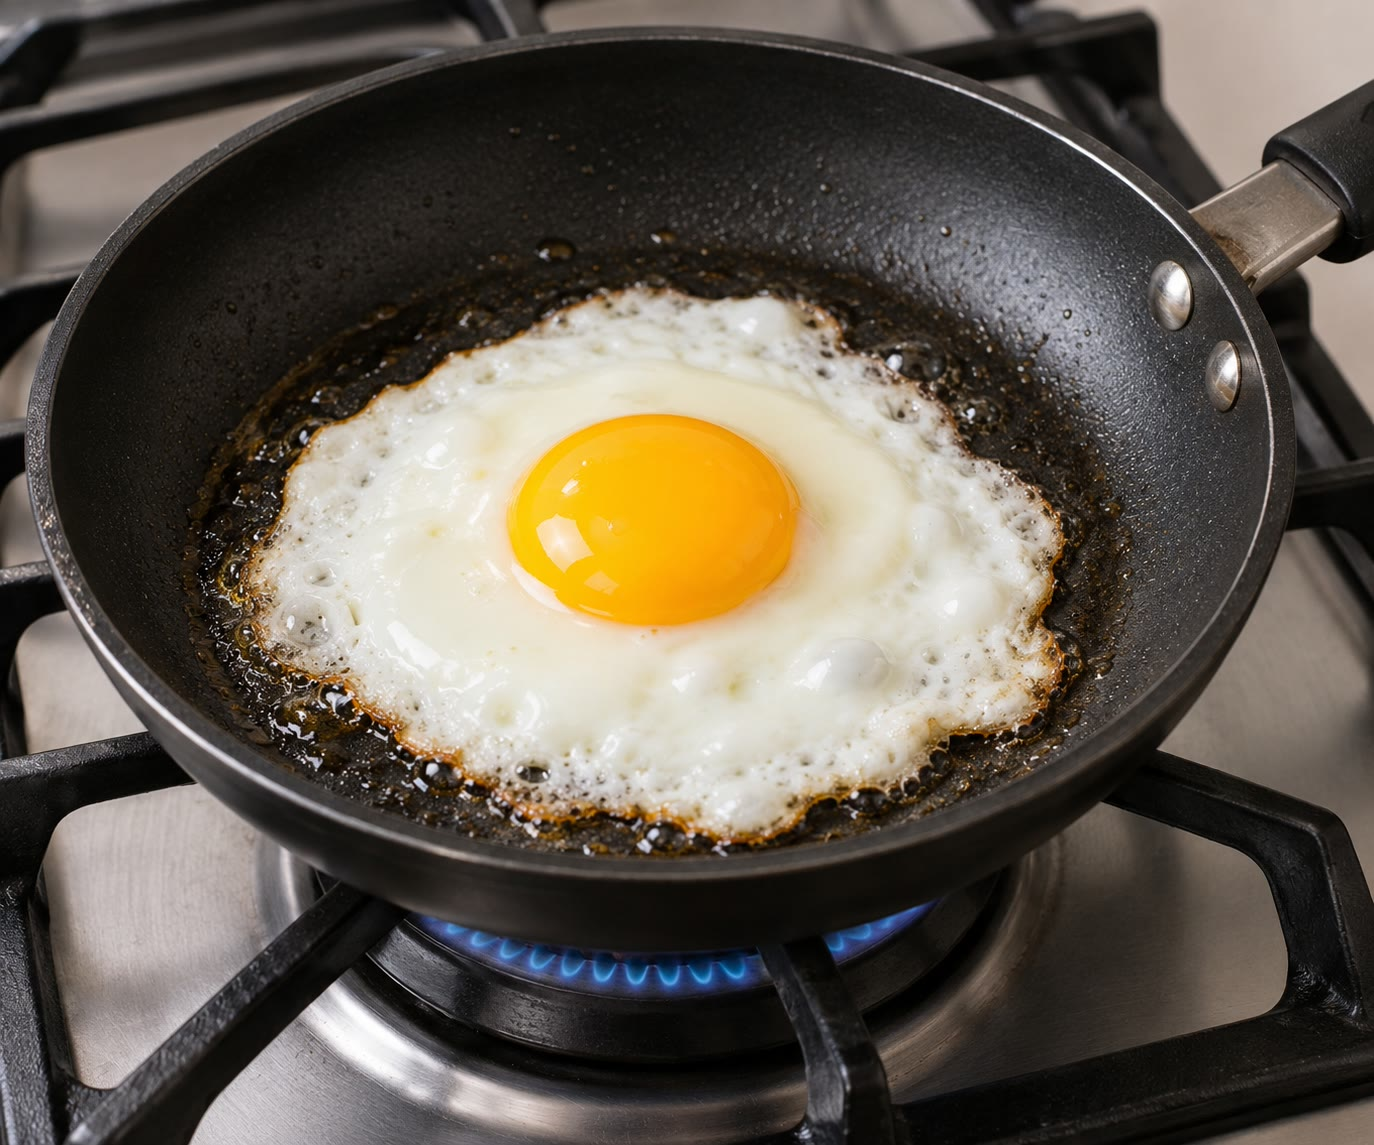
\includegraphics[width=0.55\linewidth]{images/book1/ai/g5-egg-frying.jpg}

{\small तवे पर पकता अंडा: पारदर्शी सफ़ेदी सख़्त और सफ़ेद हो गई है,
हमेशा के लिए।}
\end{omfigure}

\section{ऐसे परिवर्तन जो उलटे किए जा सकते हैं}

\begin{definition}[उत्क्रमणीय परिवर्तन]\label{def:g5:irreversible-changes:reversible}
\emph{उत्क्रमणीय परिवर्तन}\index{उत्क्रमणीय परिवर्तन} वह परिवर्तन है
जिसे उलटा किया जा सके, ताकि हमें ठीक वही वापस मिल जाए जिससे हमने शुरुआत की थी।
\end{definition}

\begin{example}[घुलना और सुखाना]\label{ex:g5:irreversible-changes:dissolve}
पानी में मिलाकर चलाई गई चीनी घुल जाती है। पानी का \omterm{def:g3:separating-mixtures:evaporate}{वाष्पन} होने दो, तो
चीनी वापस आ जाती है: वही चीनी, पहले जितनी मीठी। \omterm{def:g2:mixing-and-dissolving:dissolve}{घुलना} एक
\omterm{def:g5:irreversible-changes:reversible}{उत्क्रमणीय परिवर्तन} है।
\end{example}

\begin{example}[बर्फ़ और पानी]\label{ex:g5:irreversible-changes:ice}
बर्फ़ का टुकड़ा गरम प्लेट पर पिघलकर पानी बन जाता है; पानी को फ़्रीज़र में
रखो, तो वह फिर बर्फ़ बन जाता है। पिघलना और जमना \omterm{def:g5:irreversible-changes:reversible}{उत्क्रमणीय
परिवर्तन} हैं। (पानी क्यों पिघलता और जमता है, यह भौतिकी की पुस्तक में बताया गया है।)
\end{example}

\begin{example}[मिलाना]\label{ex:g5:irreversible-changes:mix}
बजरी में मिली रेत को फिर से चालकर अलग किया जा सकता है; गंदले पानी को
छाना जा सकता है। \omterm{def:g2:mixing-and-dissolving:mix}{मिलाना} एक \omterm{def:g5:irreversible-changes:reversible}{उत्क्रमणीय परिवर्तन} है: कुछ नया नहीं बनता, और
हिस्सों को अलग किया जा सकता है (\cref{ch:g3:separating-mixtures})।
\end{example}

\section{ऐसे परिवर्तन जो उलटे नहीं किए जा सकते}

\begin{definition}[अनुत्क्रमणीय परिवर्तन और रासायनिक परिवर्तन]\label{def:g5:irreversible-changes:chemical-change}
\emph{अनुत्क्रमणीय परिवर्तन}\index{अनुत्क्रमणीय परिवर्तन} वह परिवर्तन है
जिसे सीधे-सीधे उलटा नहीं किया जा सकता। इनमें से ज़्यादातर ऐसे परिवर्तन होते
हैं जिनमें ऐसे नए पदार्थ प्रकट होते हैं जो शुरुआत में नहीं थे: ऐसे परिवर्तन
को \emph{रासायनिक परिवर्तन}\index{रासायनिक परिवर्तन} कहते हैं।
\end{definition}

\begin{example}[छह रासायनिक परिवर्तन]\label{ex:g5:irreversible-changes:six}
\begin{itemize}
  \item \textbf{अंडा पकाना}: बहती, पारदर्शी सफ़ेदी सख़्त और सफ़ेद हो
        जाती है।
  \item \textbf{केक सेंकना}: पतला घोल एक स्पंज जैसा केक बन जाता है,
        जो बाहर से भूरा होता है और जिसमें नई गंध होती है।
  \item \textbf{\omterm{def:g4:what-a-fire-needs:burning}{जलना}}: लकड़ी राख, धुआँ, कार्बन डाइऑक्साइड और
        जलवाष्प बन जाती है।
  \item \textbf{जंग लगना}: बारिश में बाहर छोड़ा गया चमकीला लोहा एक
        परतदार नारंगी-भूरे पदार्थ, जंग, से ढक जाता है।
  \item \textbf{दूध का खट्टा होना}: कई दिन भूला रहने पर दूध गाढ़ा हो
        जाता है, उसमें गुठलियाँ बनती हैं और उससे खट्टी गंध आती है।
  \item \textbf{कटे सेब का भूरा होना}: उसका हल्के रंग का गूदा एक घंटे के
        भीतर \omterm{def:g4:air-a-mixture-of-gases:air}{हवा} में भूरा हो जाता है।
\end{itemize}
हर बार कुछ नया बना है, और जिससे हमने शुरुआत की थी उसे वापस पाने का
कोई सीधा तरीका नहीं है।
\end{example}

\begin{omfigure}
\begin{minipage}[t]{0.48\linewidth}\centering
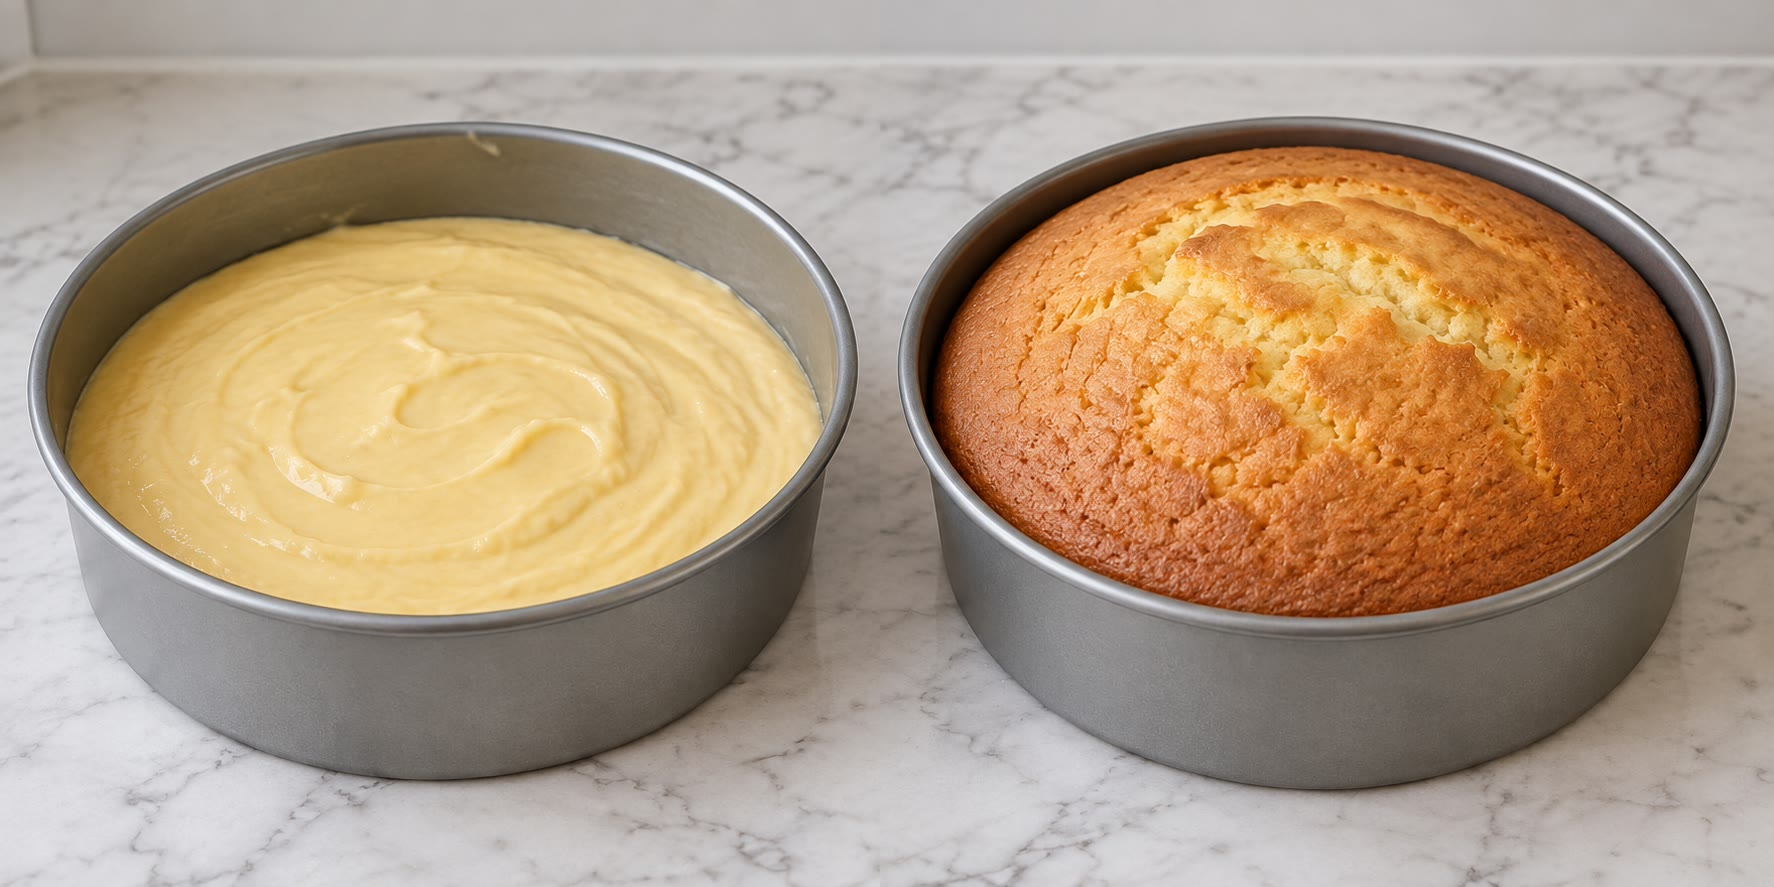
\includegraphics[width=\linewidth,height=4.6cm,keepaspectratio]{images/book1/ai/g5-cake-before-after.jpg}

{\small पहले घोल, बाद में केक: सेंकने को उलटा नहीं किया जा सकता।}
\end{minipage}\hfill
\begin{minipage}[t]{0.48\linewidth}\centering
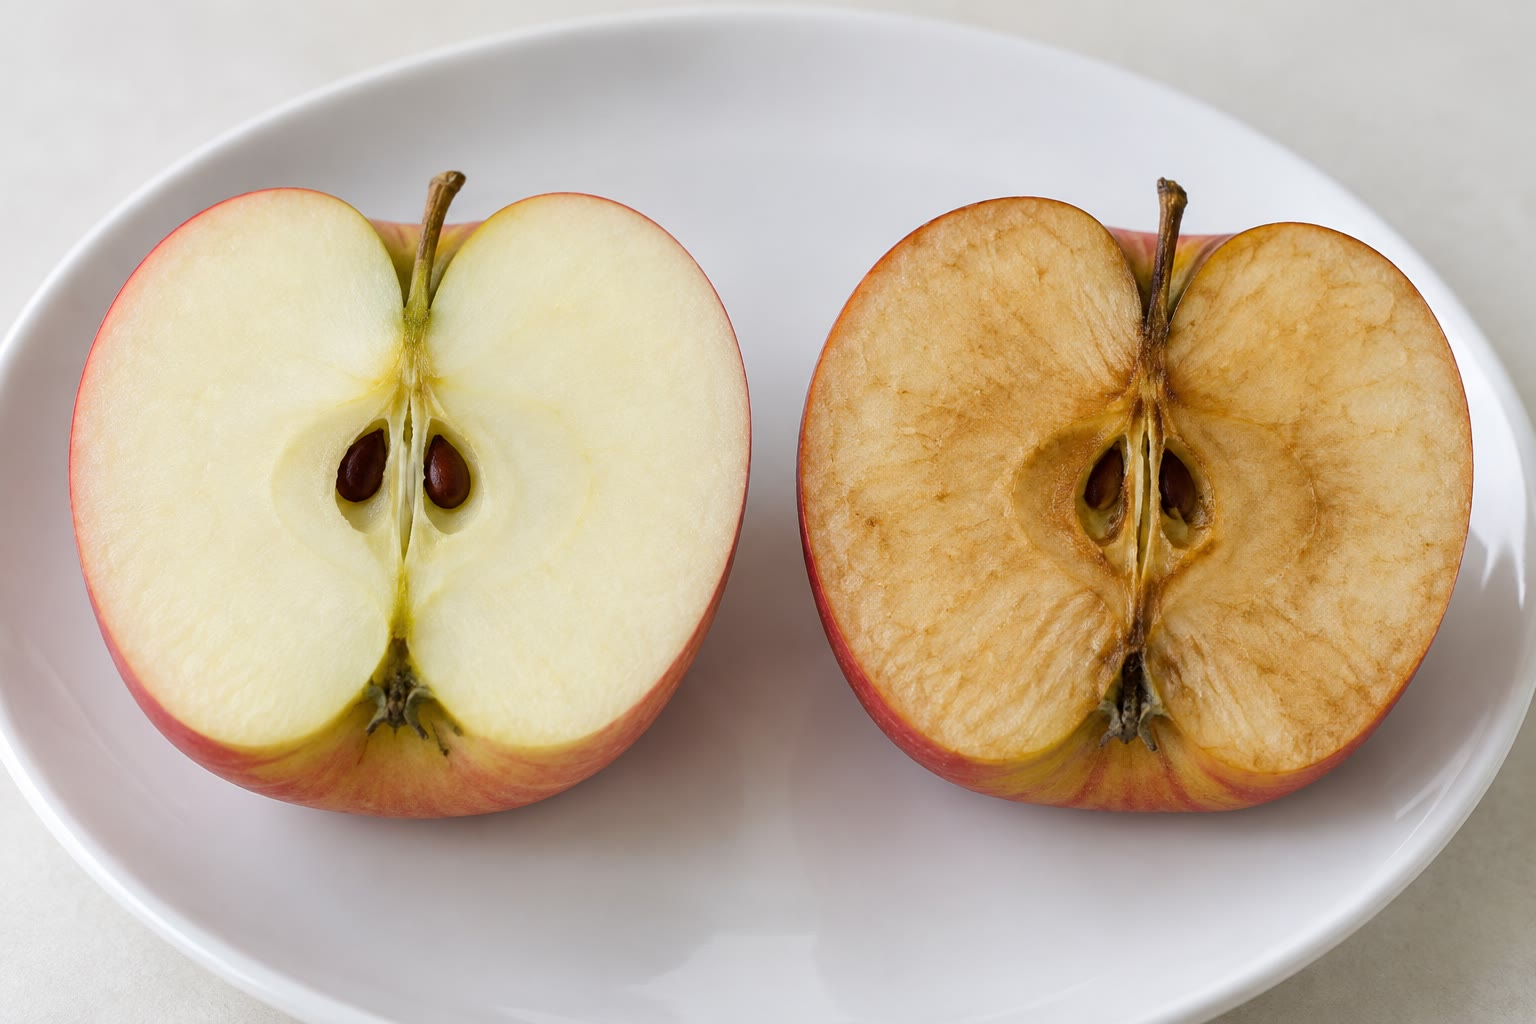
\includegraphics[width=\linewidth,height=4.6cm,keepaspectratio]{images/book1/ai/g5-apple-browning.jpg}

{\small एक ताज़ा आधा टुकड़ा, और एक घंटे \omterm{def:g4:air-a-mixture-of-gases:air}{हवा} में छोड़ा गया आधा टुकड़ा।}
\end{minipage}
\end{omfigure}

\begin{omfigure}
\begin{tikzpicture}[font=\small]
  \node[font=\small\bfseries, omDef] at (2.7,4.6) {उलटे हो सकते हैं};
  \node[font=\small\bfseries, omProp] at (9.6,4.6) {उलटे नहीं हो सकते};
  \draw[black!30] (6.1,4.9) -- (6.1,-0.3);
  % reversible pairs
  \foreach \y/\a/\b in {3.6/{चीनी + पानी}/{चीनी का पानी}, 2.0/{बर्फ़}/{द्रव पानी},
                        0.4/{रेत + बजरी}/{मिश्रण}} {
    \node[draw=omDef, fill=omDef!6, rounded corners=2pt, minimum width=2.3cm,
      minimum height=0.8cm] at (0.9,\y) {\a};
    \node[draw=omDef, fill=omDef!6, rounded corners=2pt, minimum width=2.3cm,
      minimum height=0.8cm] at (4.6,\y) {\b};
    \draw[->, thick, omDef] (2.3,\y+0.12) -- (3.25,\y+0.12);
    \draw[<-, thick, omDef] (2.3,\y-0.12) -- (3.25,\y-0.12);
  }
  % irreversible ones
  \foreach \y/\a/\b in {3.6/{कच्चा अंडा}/{पका अंडा}, 2.0/{लकड़ी}/{राख, धुआँ, गैसें},
                        0.4/{लोहा}/{जंग}} {
    \node[draw=omProp, fill=omProp!6, rounded corners=2pt, minimum width=2.0cm,
      minimum height=0.8cm] at (7.6,\y) {\a};
    \node[draw=omProp, fill=omProp!6, rounded corners=2pt, minimum width=2.9cm,
      minimum height=0.8cm] at (11.5,\y) {\b};
    \draw[->, thick, omProp] (8.8,\y) -- (9.85,\y);
  }
\end{tikzpicture}

{\small बाईं ओर: \omterm{def:g5:irreversible-changes:reversible}{उत्क्रमणीय परिवर्तन}, दोहरा तीर बताता है कि वे दोनों ओर
हो सकते हैं। दाईं ओर: \omterm{def:g5:irreversible-changes:chemical-change}{रासायनिक परिवर्तन}, केवल एक ओर।}
\end{omfigure}

\section{नया पदार्थ बनने के सुराग़}

\begin{method}[क्या यह रासायनिक परिवर्तन है? सुराग़ ढूँढो]\label{met:g5:irreversible-changes:clues}
नया पदार्थ अक्सर इनमें से किसी सुराग़ से पकड़ में आ जाता है:
\begin{enumerate}
  \item नया \textbf{रंग} (सिंकी हुई डबलरोटी के टुकड़े का भूरा रंग);
  \item बिना गरम किए किसी द्रव में किसी गैस के \textbf{बुलबुले}
        बनना (खाने के सोडे पर डाला गया सिरका);
  \item नई \textbf{गंध} (खट्टा दूध, जली डबलरोटी);
  \item \textbf{ऊष्मा या प्रकाश} निकलना (\omterm{def:g4:what-a-fire-needs:burning}{जलती} मोमबत्ती);
  \item किसी स्वच्छ द्रव में \textbf{ठोस प्रकट होना}, या गुठलियाँ बनना
        (दूध का फटना)।
\end{enumerate}
अकेला एक सुराग़ धोखा दे सकता है: उबलते पानी में बुलबुले बनते हैं, पर कुछ
नया नहीं बनता --- बुलबुले जलवाष्प हैं, और भाप ठंडी होने पर पानी वापस आ
जाता है। कई सुराग़ ढूँढो, और पूछो: क्या इसे उलटा किया जा सकता है?
\end{method}

\begin{omfigure}
\begin{tikzpicture}[font=\small]
  \foreach \k/\t in {0/{नया रंग}, 1/{गैस के बुलबुले}, 2/{नई गंध},
                     3/{ऊष्मा या प्रकाश}, 4/{ठोस प्रकट होता है}} {
    \begin{scope}[xshift=\k*3.2cm]
      \draw[omProp, line width=0.8pt, fill=omProp!5] (0,0) circle (1.0);
      \node[anchor=north, align=center] at (0,-1.15) {\t};
    \end{scope}
  }
  % 1: colour, a slice of toast half brown
  \fill[yellow!20, draw=brown!60] (-0.55,-0.5) rectangle (0.55,0.55);
  \fill[brown!55] (0,-0.5) rectangle (0.55,0.55);
  % 2: bubbles in a beaker
  \begin{scope}[xshift=3.2cm]
    \pic[transform shape, scale=0.45] at (0,-0.55) {beaker={0.7}{omWater!80}};
    \foreach \x/\y in {-0.15/-0.2,0.1/0.05,-0.05/0.25,0.18/-0.35,-0.2/0.15}
      \draw[black!55] (\x,\y) circle (0.05);
  \end{scope}
  % 3: smell, wavy lines
  \begin{scope}[xshift=6.4cm]
    \foreach \x in {-0.35,0,0.35} \draw[black!55, line width=0.8pt, decorate,
      decoration={snake, amplitude=1.5pt, segment length=6pt}] (\x,-0.6) -- (\x,0.6);
  \end{scope}
  % 4: a flame
  \begin{scope}[xshift=9.6cm]
    \fill[orange!80] (0,-0.6) .. controls (-0.45,-0.05) and (-0.15,0.35) .. (0,0.7)
      .. controls (0.15,0.35) and (0.45,-0.05) .. (0,-0.6);
    \fill[yellow!80] (0,-0.45) .. controls (-0.2,-0.1) and (-0.08,0.15) .. (0,0.3)
      .. controls (0.08,0.15) and (0.2,-0.1) .. (0,-0.45);
  \end{scope}
  % 5: solid settling in a test tube
  \begin{scope}[xshift=12.8cm]
    \pic[transform shape, scale=0.4] at (0,-0.65) {testtube={0.75}{omWater!80}};
    \fill[white, draw=black!40] (-0.08,-0.62) rectangle (0.08,-0.5);
    \foreach \x/\y in {-0.04/-0.3,0.04/-0.1,0/0.1} \fill[black!35] (\x,\y) circle (0.03);
  \end{scope}
\end{tikzpicture}

{\small पाँच सुराग़ कि शायद कोई \omterm{def:g5:irreversible-changes:chemical-change}{रासायनिक परिवर्तन} हुआ है।}
\end{omfigure}

\begin{inthelab}[खाने के सोडे पर सिरका]
शिक्षक एक बीकर की तली में एक चम्मच खाने का सोडा, एक सफ़ेद चूर्ण, रखते
हैं और उसमें थोड़ा सिरका डालते हैं। मिश्रण तुरंत सनसनाता है और झाग बनकर
ऊपर उठता है: एक गैस निकलती है, जो \omterm{def:g5:irreversible-changes:chemical-change}{रासायनिक परिवर्तन} का एक सुराग़ है। सनसनाहट
रुकने पर खाने का सोडा जा चुका होता है और सुखाकर वापस नहीं पाया जा
सकता।
\end{inthelab}

\begin{omfigure}
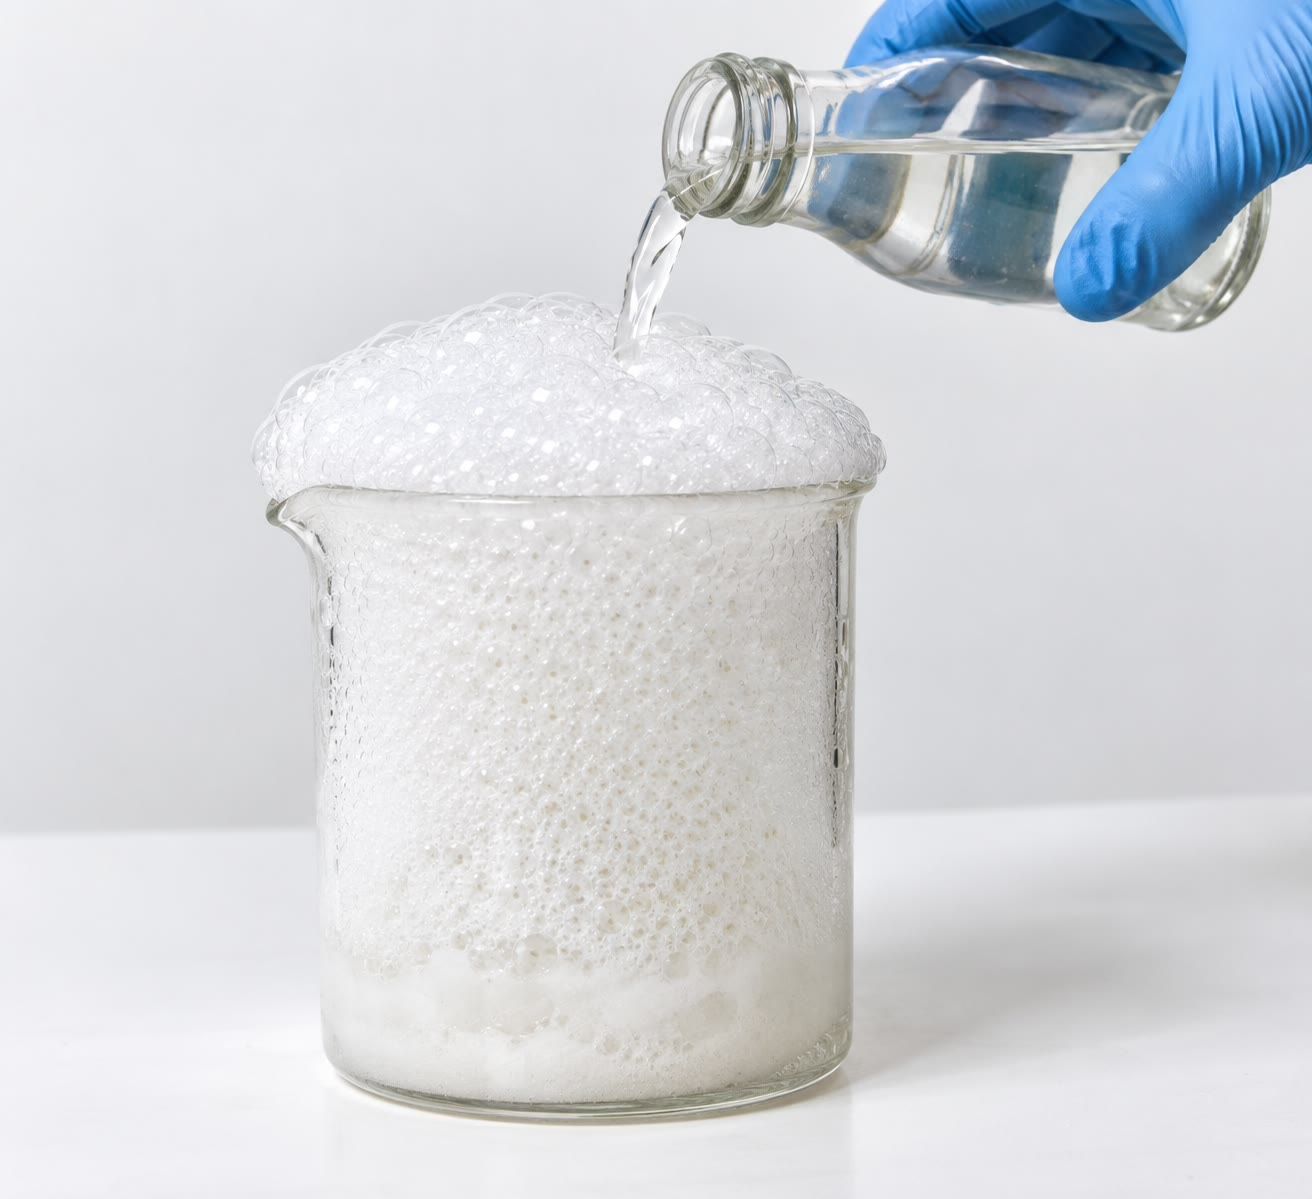
\includegraphics[width=0.5\linewidth]{images/book1/ai/g5-baking-soda-lab.jpg}

{\small खाने के सोडे पर सिरका: एक गैस निकलती है।}
\end{omfigure}

\section{उपयोगी और हानिकारक परिवर्तन}

\begin{proposition}[हमारे आस-पास के रासायनिक परिवर्तन]\label{prop:g5:irreversible-changes:around}
बहुत-से \omterm{def:g5:irreversible-changes:chemical-change}{रासायनिक परिवर्तन} उपयोगी हैं: खाना पकाना, डबलरोटी सेंकना, घर
गरम करने के लिए गैस जलाना, प्लास्टर या सीमेंट का जमकर सख़्त होना। कुछ
नुक़सान करते हैं: लोहे में जंग लगना, खाना ख़राब होना, लकड़ी का सड़ना। हम
इन्हें उलटा नहीं कर सकते, पर इन्हें धीमा कर सकते हैं:
\begin{itemize}
  \item फ़्रिज की ठंडक में खाना ज़्यादा दिन टिकता है;
  \item पेंट या तेल की परत \omterm{def:g4:air-a-mixture-of-gases:air}{हवा} और पानी को लोहे से दूर रखती है;
  \item नींबू का रस छिड़का गया कटा सेब ज़्यादा धीरे भूरा होता है।
\end{itemize}
\end{proposition}

\begin{omfigure}
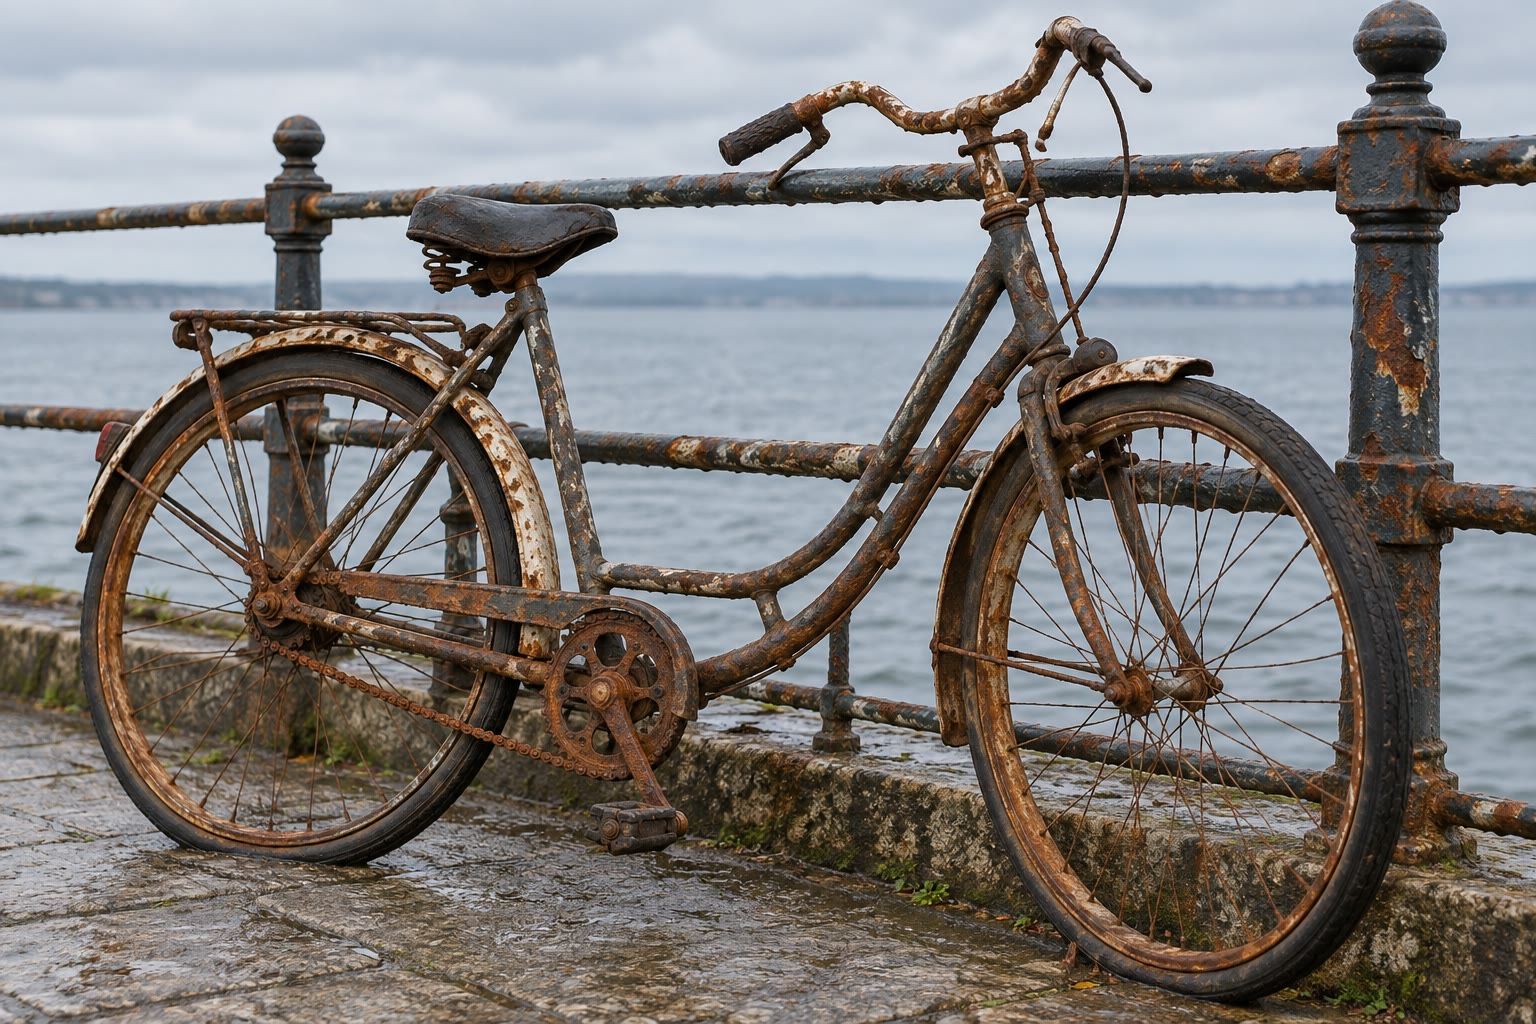
\includegraphics[width=0.55\linewidth]{images/book1/ai/g5-rusty-bicycle.jpg}

{\small बरसों तक बारिश में बाहर छोड़ी गई साइकिल: लोहे में जंग लग गया है।}
\end{omfigure}

\begin{remark}[उलटा हो सकता है, पर सीधे-सीधे नहीं]\label{rem:g5:irreversible-changes:not-simply}
``उलटा नहीं किया जा सकता'' का अर्थ है कि ठंडा करने या सुखाने जैसा कोई
सीधा रास्ता वापस नहीं है। रसायनज्ञ कभी-कभी जंग को फिर से लोहा बना सकते
हैं, पर केवल भट्ठी और नए पदार्थों की मदद से: वह एक और \omterm{def:g5:irreversible-changes:chemical-change}{रासायनिक
परिवर्तन} है, उलटा करना नहीं।
\end{remark}

\section{अभ्यास}

\begin{exercise}[$\star$]\label{exo:g5:irreversible-changes:1}
बताओ कि हर परिवर्तन उलटा किया जा सकता है या नहीं: चॉकलेट पिघलाना, तीली
जलाना, पानी में नमक घोलना, डबलरोटी सेंकना।
\end{exercise}

\begin{exercise}[$\star$]\label{exo:g5:irreversible-changes:2}
\omterm{def:g5:irreversible-changes:chemical-change}{रासायनिक परिवर्तन} क्या है? रसोई से दो उदाहरण दो।
\end{exercise}

\begin{exercise}[$\star$]\label{exo:g5:irreversible-changes:3}
पानी में नमक घोला गया है। नमक को वापस कैसे पाया जा सकता है? क्या \omterm{def:g2:mixing-and-dissolving:dissolve}{घुलना}
एक \omterm{def:g5:irreversible-changes:reversible}{उत्क्रमणीय परिवर्तन} है?
\end{exercise}

\begin{exercise}[$\star$]\label{exo:g5:irreversible-changes:4}
दूध खट्टा होने पर तुम्हें \omterm{def:g5:irreversible-changes:chemical-change}{रासायनिक परिवर्तन} का कौन-सा सुराग़ दिखता है?
दो बताओ।
\end{exercise}

\begin{exercise}[$\star$]\label{exo:g5:irreversible-changes:5}
दो स्तंभों वाला चित्र देखो। किन परिवर्तनों पर दोहरा तीर है? दोहरे तीर
का क्या अर्थ है?
\end{exercise}

\begin{exercise}[$\star$]\label{exo:g5:irreversible-changes:6}
साइकिल की चेन में तेल क्यों डाला जाता है? तेल किस \omterm{def:g5:irreversible-changes:chemical-change}{रासायनिक परिवर्तन} को
धीमा करता है?
\end{exercise}

\begin{exercise}[$\star$]\label{exo:g5:irreversible-changes:7}
खाने के सोडे पर सिरका डालने पर सनसनाहट होती है। यह कौन-सा सुराग़ है?
\end{exercise}

\begin{exercise}[$\star$]\label{exo:g5:irreversible-changes:8}
एक उपयोगी \omterm{def:g5:irreversible-changes:chemical-change}{रासायनिक परिवर्तन} और एक हानिकारक \omterm{def:g5:irreversible-changes:chemical-change}{रासायनिक परिवर्तन} का नाम बताओ।
\end{exercise}

\begin{exercise}[$\star$]\label{exo:g5:irreversible-changes:9}
हम दूध को फ़्रिज में क्यों रखते हैं?
\end{exercise}

\begin{exercise}[$\star\star$]\label{exo:g5:irreversible-changes:10}
उबलने पर पानी में बुलबुले बनते हैं। क्या उबलना एक \omterm{def:g5:irreversible-changes:chemical-change}{रासायनिक परिवर्तन} है?
समझाओ कि एक अकेला सुराग़ काफ़ी क्यों नहीं है।
\end{exercise}

\begin{exercise}[$\star\star$]\label{exo:g5:irreversible-changes:11}
टॉम कहता है: ``मोमबत्ती \omterm{def:g4:what-a-fire-needs:burning}{जलती} है तो मोम बस बर्फ़ की तरह पिघलकर बह जाता है।''
दो सुराग़ों से समझाओ कि मोमबत्ती का \omterm{def:g4:what-a-fire-needs:burning}{जलना} एक \omterm{def:g5:irreversible-changes:chemical-change}{रासायनिक परिवर्तन} है,
केवल पिघलना नहीं।
\end{exercise}
